%% Sample file $Id: PBML_article.tex 134 2010-07-01 19:28:04Z popel $
\documentclass{pbml}
%\documentclass[nofonts]{pbml} % for XeLaTeX without Pagella and DejaVu fonts
%\documentclass[color]{pbml} % for color images and hypertext links
% test

% This is a sample file for the PBML article.
% You can compile it with (ordered by preference)
%  1. XeLaTeX with installed fonts TeX Gyre Pagella and DejaVu
%  2. XeLaTeX without the fonts -> you must use \documentclass[nofonts]{pbml}
%  3. pdfLaTeX
%
% In all three methods, you can use Unicode (utf8) encoding for special letters
% (so instead of na\"{i}ve you can write directly naïve).
% Note that with methods 2 and 3, your output will be slightly DIFFERENT than
% our final print version (different line breaks and page breaks).
% See the end of this file for more information.

% Packages
% ========
% In this place you can load required packages by the \usepackage commands.
% The following packages are loaded automatically by the class:
% euler    (for math fonts)
% graphicx (for inclusion of images)
% multicol (for multicolumn typesetting)
% natbib   (for bibliography citations)
% amssymb  (for various symbols)
% If XeLaTeX is used, fontspec and xltxtra are loaded as well.
\usepackage{algorithmic}
\usepackage{amsmath}
\usepackage{tikz,gnuplot-lua-tikz} 

% Definitions
% ===========
% You can use your own macros defined by \newcommand, \providecommand,
% \DeclareRobustCommand (or even by \def) as well as environments declared by
% \newenvironment. You can also use \newcounter in order to declare your own counters.

\begin{document}

% Document title and authors
% ==========================
% Due to journal organization, the article title and authors must be specified
% AFTER \begin{document}. Note that \subtitle is not allowed anymore due to
% problems with indexing in science databases. If needed use colon in the title.

\title{A Comparison of Synchronous-CFG \titlelinebreak{} Decoder Implementations}


% Now put the affiliated institutes first, then author names and the labels
% of their institutes in the "institute" field. The order of institutes and
% authors printed below the title will be the same as the order of your commands.
% Each author can be associated with more than one institute.
% One author must be chosen as the "corresponding author" (using attribute
% corresponding) and his or her email and full address must be provided.
% PLEASE, use Unicode (utf8) encoding (e.g ï instead of \"{i}).

\institute{label1}{University of Edinburgh}
\institute{label2}{Center for Language and Speech Processing, Johns Hopkins University}
\institute{label3}{Carnegie Mellon University}

\author{
  firstname=Hieu,
  surname=Hoang,
  institute=label1,
}
\author{
  firstname=Matt,
  surname=Post,
  institute=label2,
}
\author{
  firstname=Kenneth,
  surname=Heafield,
  institute=label1,
}
\author{
  firstname=Eva,
  surname=Hasler,
  institute=label1,
}
\author{
  firstname=Phil,
  surname=Williams,
  institute=label1,
}
\author{
  firstname=Barry,
  surname=Haddow,
  institute=label1,
}
\author{
  firstname=Chris,
  surname=Dyer,
  institute=label3,
}
\author{
  firstname=Philipp,
  surname=Koehn,
  institute=label1,
}

% If all authors belong to the same institute, you can use simpler syntax:
% \institute{}{Charles University in Prague, Faculty of Mathematics and Physics, Institute of Formal and Applied Linguistics}
% \author{firstname=Humpty, surname=Dumpty}
% \author{firstname=Mock, surname=Turtle,
%   corresponding=yes,
%   email={turtle@seacoast.wl},
%   address={Institute of Formal and Applied Linguistics\\
%            Faculty of Mathematics and Physics,\\
%            Charles University in Prague\\
%            Malostranské náměstí 25\\
%            118 00 Praha 1, Czech Republic}}
% \author{firstname=Cheshire, surname=Cat}


% The title and authors' names are used in the running head. If they are
% long, you should define short versions. These definitions are optional. You
% define them only if they are needed. The example follows:
\shorttitle{SCFG Decoder Implementations}
\shortauthor{H. Dumpty, M. Turtle, C. Cat}

% Now print the title by:
\PBMLmaketitle


% Abstract
% ========
% The abstract is placed within the "abstract" environment. It is a mandatory
% part of the article. PLEASE, do not use your own macros in abstract, if possible.

\begin{abstract}
Best practise for developing a SMT decoder has progressed enormously since the initial release of the Moses decoder in 2006. The emergence of syntax-inspired models, sparse features and more features, have been the driver for the major changes in the framework of the decoder.

In this paper, we describe the changes in the Moses decoder to support such changes. How we have updated the decoder, and dependent programs, while preserving the rich features in the toolkit. Particular emphasis will be place in describing the feature function framework.

The open-source community has also changed from the dominance of phrase-based model and virtual Moses monopoly, to a situation where syntactic models are leading the research agenda, and other projects such as cdec and Joshua have equal prominence.
We take this opportunity to compare the implementations of these other decoders with Moses. We find that there are many similarities between the decoders, but also some surprising differences in implementation of even very fundamental features in each decoder.

\end{abstract}

\section{Introduction}
% The body of the article
% =======================
% The PBML class is modelled after the standard article class. This means
% that you can use almost everything that is allowed in articles as described
% in the textbooks of LaTeX. We support sectioning commands \section,
% \subsection and \subsubsection.

% In addition to the \cite command, you can use natbib style of citations.
% PLEASE, use \citet instead of \cite if the author names are part of the sentence.
%\citet{PDT2} show \ldots \\ % This renders as "Hajič et al. (2006) show" instead of "(Hajič et al., 2006) show".
%\ldots tree-based annotation (e.g.~\citealp{PDT2}).

In terms of extensibility, the Moses\cite{koehn-EtAl:2007:PosterDemo} decoder was a vast improvement over its immediate predecessor, Pharoah\cite{Koehn:Pharaoh:2004}. 

Moses allows multiple translation models and language models instances and implementations. Allowing multiple instances has enabled researchers to combine multiple datasets in novel ways, as well as the use of secondary models on linguistic information\cite{Koehn:Philipp:2007, Sennrich:Rico:2011,Koehn:Philipp:2012}. Allowing multiple implementations has spurred on the developments of smaller, faster, better implementation of language models and phrase tables\cite{talbot-osborne:2007:ACLMain, Heafield-kenlm, Junczys-Dowmunt:Marcin:2012}.

However, a direction of machine translation research in the last few years has been improving translation quality with the addition of ad-hoc feature functions outside of the translation model and language model types. Also, the use of sparse features during decoding has also been popular. Research such as \cite{chiang-knight-wang:2009:NAACLHLT09, cherry:2013:NAACL-HLT} typifies this approach.

Enabling ad-hoc features and sparse features requires a more extensible framework that incorporate feature functions into the decoder.

It also required tuning algorithms which are able to deal with a large number of features. It is generally known that MERT is unstable with a large number of features.

This paper describes the changes to the Moses decoder in order to incorporate more feature functions, and compares it with that implemented in cdec\cite{Dyer_etal_2010} and Joshua\cite{Joshua-Decoder}.

\section{Feature Function Framework}
\subsection{Old Framework}

The built-in feature functions in the phrase-based models are:
\begin{itemize}
  \item Translation model
  \item Language model
  \item Distortion model
  \item Lexicalized reordering model
  \item Word penalty
  \item Unknown word penalty
\end{itemize}

The hierarchical and syntax model also uses these feature functions, except for the distortion and lexicalized reordering model.

Each feature function is implemented in a separate class, with no common class hierarchy. The initialisation and evaluation of each feature function was entirely bespoked.

Feature function state information is an essential component of the search procedure in decoding. State information control hypothesis recombination, enabling the decoder to effectively search through many more hypotheses than it actually has. State information is emitted from stateful feature functions.

The state information in Moses has evolved since inception. Initially, state information was only available from language models, therefore, only language models states are compared, Figure~\ref{algo:CompareHypoStates}.

\begin{figure} [h!]
\small 
\begin{algorithmic}
\REQUIRE hypothesis $a$, hypothesis b

       \IF {coverage of a != coverage of b }
	\RETURN not equal
       \ENDIF
       
        \FORALL {LM state s}
          \IF {state s of hypothesis a != state s for hypothesis b}
	    \RETURN not equal
	 \ENDIF
        \ENDFOR
        \RETURN equal

\end{algorithmic}
\caption{Comparing Hypothesis States (old framework)}
\label{algo:CompareHypoStates}
\end{figure} 

\subsection{New Framework}        
 All feature functions inherit indirectly from the class \emph{FeatureFunction}, which provides basic services to all feature functions such as storing the name and number of dense features, and providing a central repository of all feature functions.

A feature function can be stateless or stateful, depending on whether it inherits from \emph{StatelessFeatureFunction} or \emph{StatefulFeatureFunction}, respectively.

The state comparison routine of Figure~\ref{algo:CompareHypoStates} evolved to compare the state of all stateful feature functions, Figure~\ref{algo:CompareHypoStates.new}.

\begin{figure} [h!]
\small 
\begin{algorithmic}
\REQUIRE hypothesis $a$, hypothesis b

       \IF {coverage of a != coverage of b }
	\RETURN not equal
       \ENDIF
       
        \FORALL {feature function state s}
          \IF {state s of hypothesis a != state s for hypothesis b}
	    \RETURN not equal
	 \ENDIF
        \ENDFOR
        \RETURN equal

\end{algorithmic}
\caption{Comparing Hypothesis States (new framework)}
\label{algo:CompareHypoStates.new}
\end{figure} 
        
\subsection{cdec and Joshua}
cdec and Joshua both have modern feature function frameworks similar to the Moses new framework. cdec has no distinction between stateful and stateless features; stateless features have zero size states.

\section{Hypothesis and Translation Rule Evaluation}
\subsection{Old Framework}
The range of feature functions are hardcoded when evaluating the scores of hypotheses and translation rules. Translation rules are evaluated according to Equation~\ref{eq:translation rule score}:
\begin{equation}
  score = \sum_{m \in T} \sum_{i \in m} (\lambda_{m,i} * score_{m,i}) + \sum_{l  \in L} (\lambda_l * score_i) + \lambda_{wp} * words
\label{eq:translation rule score}
\end{equation}
where $T$ is the set of translation models, and $L$ is the set of sequence models, $\lambda_{m,i}$ is the i'th weight for translation model $m$, $\lambda_l$ is the weight for language model $l$, $\lambda_{wp}$ is the word penalty weight.

Similarly, hypotheses are evaluated as follows, Equation~\ref{eq:hypothesis rule score}:
\begin{equation}
\begin{split}
 score & =  \sum_{m \in T} \sum_{i \in m} (\lambda_{m,i} * score_{m,i}) \\
    & + \sum_{l \in L} (\lambda_l * score_l) \\
    & + \lambda_{wp} * words \\
    & + \lambda_d * score_d \\
    & + \sum_{m \in R} \sum_{i \in m} (\lambda_{m,i} * score_{m,i})  \\
    & + score_{future} \\
\label{eq:hypothesis rule score}
\end{split}
\end{equation}
where $\lambda_d$ is the distortion weight, and $R$ is the set of lexicalized reordering models, and $score_{future}$ is the estimate of the score to completion for the hypothesis.

When adding a new feature function, its scores would not be included in the translation rule or hypothesis scores until the implementation of Equation~\ref{eq:translation rule score} and Equation~\ref{eq:hypothesis rule score} are update.

%Translation rule always evaluated occurs before decoding, either during loading of the feature function, or just before the translation rule is used in decoding.

%Hypotheses are evaluated when they are created during the search process.

\subsection{New Framework}
The new framework better supports the creation of arbitrary feature functions by generalizing all code that deals with feature functions.

Equation~\ref{eq:translation rule score} becomes Equation~\ref{eq:translation rule score.new}
\begin{equation}
  score = \sum_{m \in FF} \sum_{i \in m} (\lambda_{m,i} * score_{m,i})
\label{eq:translation rule score.new}
\end{equation}
where $FF$ is the set of feature functions.

Similarly, Equation~\ref{eq:hypothesis rule score} becomes Equation~\ref{eq:hypothesis rule score.new}:
\begin{equation}
  score =  \sum_{m \in FF} \sum_{i \in m} (\lambda_{m,i} * score_{m,i})
	  + score_{future}
\label{eq:hypothesis rule score.new}
\end{equation}

Furthermore, there are three stages during decoding where each feature function can be evaluated:
\begin{enumerate}
    \item During creation of translation rules. Access to the words in the source and target side of translation rule.
    \item Just before decoding. Access to the entire source sentence to be decoded.
    \item During decoding. Access to the context information is available, containing the hypotheses create to translate the sentence so far. The exact information contained in the hypotheses is dependent on whether the formalism used.
\end{enumerate}
At each stage, a different range of information is available to the feature function to access for information. Scores that are evaluated at stage (1) can be cached and reused inter-sentence. Scores evaluted during stage (2) and (3) cannot be cached as they depend on the entire source sentence. Therefore, it is more efficient to evaluate as early as possible.

Each feature function can override any or all of the methods to evaluate at each of these stage. For example. a simple word penalty feature would typically implement its evaluation in stage (1) as access to the translation rule is sufficient information to allow it to evaluate the word penalty score.

On the other hand, a feature that depends on the bag of words of the input sentence would override the method for stage (2).

Stateful features need to override stage (3). Features that depend on the segmentation of the input sentence also need to override this stage. 

The most efficient way to implement language models is to override stage (1) and (3). As a stateful feature, it must override stage (3) to access adjacent target words to score overlapping n-grams. However, it is able to score the n-grams within each translation rule, and also calculate the estimated future cost, without the context. By evaluating the stateless portion of the language model score during stage (1) mitigate these score from having to be re-evaluated each time the translation rule is applied. This behaviour codify the existing practises by building the framework to support it, alllowing other feature function to take advantage of this efficient mechanism.

Additionally, some feature functions do not override any of the stages. These feature is so intertwined with the search operation that their scores are set by search operation themselves. The feature function exist as an identifier to locate the score. Features functions such as the translation models, unknown word penalty, and generation models score fall into this category.

\subsection{cdec and Joshua}
Moses implements a one-pass search strategy. All feature functions are evaluated when a hypothesis is created.

Joshua and cdec employs a multi-pass search strategy to translate each sentence. Each pass creates a hypergraph that is used as the input for the next pass. Both decoders evaluates stateless feature functions in the first pass, then stateful feature functions in the second.

cdec also supports an arbitrary number of passes, feature functions exactly to a particular pass.

\section{File Format}
\subsection{Old Framework}
Each feature function also required a separate section in the configuration (moses.ini) file to be created, along with the code to read the new section. For example, translation models are specified in the section
\begin{verbatim}
     [ttable-file]
\end{verbatim}
Language models in
\begin{verbatim}
     [lmodel-file]
\end{verbatim}
Furthermore, feature function also need a separate weight section, for example, for translation models:
\begin{verbatim}
     [weight-t]
\end{verbatim}
and language models:
\begin{verbatim}
     [weight-l]
\end{verbatim}
New feature functions need to create and manage their own specification and sections.

The features that can be tuned by MERT is also hardcoded in the tuning script. The MERT script has to be altered every time a new feature function is integrated into Moses.

\subsection{New Framework}
The configuration file format has been changed to minimize the amount of boilerplate code necessary when adding new feature functions. All feature functions are declared in the configuration file in the section
\begin{verbatim}
  [feature]
\end{verbatim}
In the fixed format
\begin{verbatim}
  Feature-Name [key=value]*
\end{verbatim}
For example,
\begin{verbatim}
  KENLM factor=0 path=lm.arpa order=5
\end{verbatim}
Similarly, all dense \emph{weights} are put into the section
\begin{verbatim}
  [weight]
\end{verbatim}
In the fixed format
\begin{verbatim}
  Feature-Instance= [value]*
\end{verbatim}
Weights for sparse features are in separate file referenced by the section
\begin{verbatim}
  [weight-file]
\end{verbatim}
in the format
\begin{verbatim}
  Feature-Instance feature value
\end{verbatim}
  
\section{Sparse Feature Function}

Sparse features contain scores that may only be present occasionally. Also, there may be many more sparse features than dense features. There are typically 14 scores from five feature functions in a standard phrase-based model and 7 scores in a hierarchical phrase-based model. There may be millions of sparse score in a system with sparse features. However, only a few will be present in a particular hypothesis.

This presents efficiency challenges which each decoder has attempted to solve in a different way.

\subsection{Moses}
Moses explicitly implements both dense and sparse features. Each score must be identifiable as one or the other.
The intuition behind this is that most systems will still contain dense features. Therefore, it would be more efficient to use dedicated dense vectors for these scores.

A sparse feature map was added to handle sparse scores.

\subsection{cdec}
cdec eschew the dense and sparse hybrid approach and implement only sparse maps. Dense features can still be modelled in the framework with sparse features, with some loss of efficiency.

To improve speed and memory usage, hypotheses only store deltas of feature differences with antecedent hypotheses.

\subsection{Joshua}
As with cdec, Joshua only supports sparse features, however, it uses a different strategy to improve efficiency.

Hypotheses only retain the weighted sum of the feature scores. They do not retain the individual score components unless required, for example, in the n-best list. The intuition behind this approach is that the score breakdown is only required in some situations such as producing n-best lists for tuning. In most other circumstances, they can be traded for better performance.
  
\section{Results}

Given the same formalism and model data, the results from the decoders are comparable, after
adjusting for scaling differences and constants. Figure~\ref{fig:model} shows the comparison of
model scores and BLEU scores for a hierarchical model. Moses and cdec are roughly comparable in
terms of speed. Also, Moses and cdec converges to roughly the same model scores, while Joshua makes
more search errors. 

\begin{figure}
%run report.gnuplot to update these.
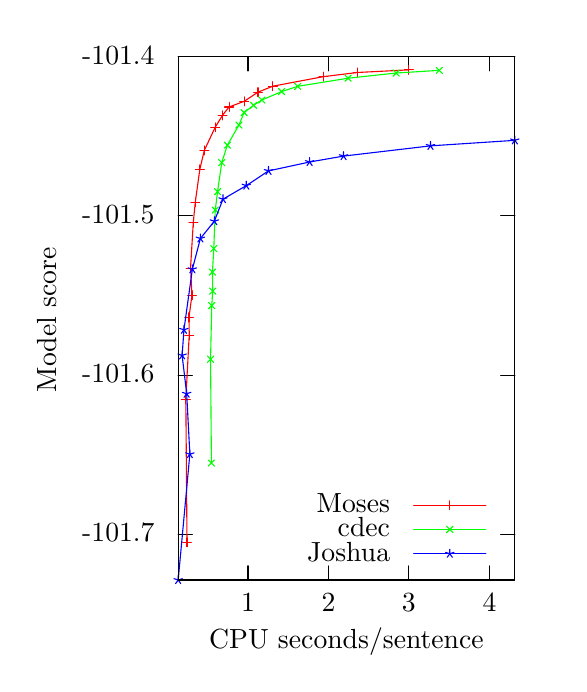
\begin{tikzpicture}[gnuplot]
%% generated with GNUPLOT 4.6p1 (Gentoo revision r0) (Lua 5.1; terminal rev. 99, script rev. 100)
%% Tue 02 Jul 2013 03:45:00 PM BST
\path (0.000,0.000) rectangle (6.700,8.000);
\gpcolor{color=gp lt color border}
\gpsetlinetype{gp lt border}
\gpsetlinewidth{1.00}
\draw[gp path] (1.872,1.565)--(2.052,1.565);
\draw[gp path] (6.147,1.565)--(5.967,1.565);
\node[gp node right] at (1.688,1.565) {-101.7};
\draw[gp path] (1.872,3.587)--(2.052,3.587);
\draw[gp path] (6.147,3.587)--(5.967,3.587);
\node[gp node right] at (1.688,3.587) {-101.6};
\draw[gp path] (1.872,5.609)--(2.052,5.609);
\draw[gp path] (6.147,5.609)--(5.967,5.609);
\node[gp node right] at (1.688,5.609) {-101.5};
\draw[gp path] (1.872,7.631)--(2.052,7.631);
\draw[gp path] (6.147,7.631)--(5.967,7.631);
\node[gp node right] at (1.688,7.631) {-101.4};
\draw[gp path] (2.758,0.985)--(2.758,1.165);
\draw[gp path] (2.758,7.631)--(2.758,7.451);
\node[gp node center] at (2.758,0.677) { 1};
\draw[gp path] (3.780,0.985)--(3.780,1.165);
\draw[gp path] (3.780,7.631)--(3.780,7.451);
\node[gp node center] at (3.780,0.677) { 2};
\draw[gp path] (4.802,0.985)--(4.802,1.165);
\draw[gp path] (4.802,7.631)--(4.802,7.451);
\node[gp node center] at (4.802,0.677) { 3};
\draw[gp path] (5.825,0.985)--(5.825,1.165);
\draw[gp path] (5.825,7.631)--(5.825,7.451);
\node[gp node center] at (5.825,0.677) { 4};
\draw[gp path] (1.872,7.631)--(1.872,0.985)--(6.147,0.985)--(6.147,7.631)--cycle;
\node[gp node center,rotate=-270] at (0.246,4.308) {Model score};
\node[gp node center] at (4.009,0.215) {CPU seconds/sentence};
\node[gp node right] at (4.679,1.935) {Moses};
\gpcolor{color=gp lt color 0}
\gpsetlinetype{gp lt plot 0}
\draw[gp path] (4.863,1.935)--(5.779,1.935);
\draw[gp path] (1.984,1.465)--(1.969,3.282)--(2.012,4.094)--(2.009,4.323)--(2.047,4.603)%
  --(2.029,4.947)--(2.064,5.530)--(2.089,5.783)--(2.147,6.202)--(2.204,6.442)--(2.342,6.735)%
  --(2.435,6.887)--(2.518,6.993)--(2.709,7.064)--(2.886,7.181)--(3.074,7.257)--(3.717,7.378)%
  --(4.151,7.431)--(4.802,7.464);
\gpsetpointsize{4.00}
\gppoint{gp mark 1}{(1.984,1.465)}
\gppoint{gp mark 1}{(1.969,3.282)}
\gppoint{gp mark 1}{(2.012,4.094)}
\gppoint{gp mark 1}{(2.009,4.323)}
\gppoint{gp mark 1}{(2.047,4.603)}
\gppoint{gp mark 1}{(2.029,4.947)}
\gppoint{gp mark 1}{(2.064,5.530)}
\gppoint{gp mark 1}{(2.089,5.783)}
\gppoint{gp mark 1}{(2.147,6.202)}
\gppoint{gp mark 1}{(2.204,6.442)}
\gppoint{gp mark 1}{(2.342,6.735)}
\gppoint{gp mark 1}{(2.435,6.887)}
\gppoint{gp mark 1}{(2.518,6.993)}
\gppoint{gp mark 1}{(2.709,7.064)}
\gppoint{gp mark 1}{(2.886,7.181)}
\gppoint{gp mark 1}{(3.074,7.257)}
\gppoint{gp mark 1}{(3.717,7.378)}
\gppoint{gp mark 1}{(4.151,7.431)}
\gppoint{gp mark 1}{(4.802,7.464)}
\gppoint{gp mark 1}{(5.321,1.935)}
\gpcolor{color=gp lt color border}
\node[gp node right] at (4.679,1.627) {cdec};
\gpcolor{color=gp lt color 1}
\gpsetlinetype{gp lt plot 1}
\draw[gp path] (4.863,1.627)--(5.779,1.627);
\draw[gp path] (2.294,2.471)--(2.283,3.789)--(2.298,4.471)--(2.311,4.655)--(2.307,4.896)%
  --(2.324,5.194)--(2.343,5.684)--(2.372,5.917)--(2.425,6.287)--(2.497,6.508)--(2.643,6.763)%
  --(2.709,6.921)--(2.829,7.014)--(2.934,7.081)--(3.185,7.188)--(3.390,7.255)--(4.029,7.358)%
  --(4.641,7.424)--(5.188,7.458);
\gppoint{gp mark 2}{(2.294,2.471)}
\gppoint{gp mark 2}{(2.283,3.789)}
\gppoint{gp mark 2}{(2.298,4.471)}
\gppoint{gp mark 2}{(2.311,4.655)}
\gppoint{gp mark 2}{(2.307,4.896)}
\gppoint{gp mark 2}{(2.324,5.194)}
\gppoint{gp mark 2}{(2.343,5.684)}
\gppoint{gp mark 2}{(2.372,5.917)}
\gppoint{gp mark 2}{(2.425,6.287)}
\gppoint{gp mark 2}{(2.497,6.508)}
\gppoint{gp mark 2}{(2.643,6.763)}
\gppoint{gp mark 2}{(2.709,6.921)}
\gppoint{gp mark 2}{(2.829,7.014)}
\gppoint{gp mark 2}{(2.934,7.081)}
\gppoint{gp mark 2}{(3.185,7.188)}
\gppoint{gp mark 2}{(3.390,7.255)}
\gppoint{gp mark 2}{(4.029,7.358)}
\gppoint{gp mark 2}{(4.641,7.424)}
\gppoint{gp mark 2}{(5.188,7.458)}
\gppoint{gp mark 2}{(5.321,1.627)}
\gpcolor{color=gp lt color border}
\node[gp node right] at (4.679,1.319) {Joshua};
\gpcolor{color=gp lt color 2}
\gpsetlinetype{gp lt plot 2}
\draw[gp path] (4.863,1.319)--(5.779,1.319);
\draw[gp path] (1.872,0.985)--(2.020,2.583)--(1.980,3.351)--(1.922,3.838)--(1.945,4.163)%
  --(2.052,4.932)--(2.154,5.323)--(2.331,5.542)--(2.441,5.822)--(2.737,5.994)--(3.019,6.181)%
  --(3.541,6.294)--(3.972,6.369)--(5.076,6.499)--(6.147,6.569);
\gppoint{gp mark 3}{(1.872,0.985)}
\gppoint{gp mark 3}{(2.020,2.583)}
\gppoint{gp mark 3}{(1.980,3.351)}
\gppoint{gp mark 3}{(1.922,3.838)}
\gppoint{gp mark 3}{(1.945,4.163)}
\gppoint{gp mark 3}{(2.052,4.932)}
\gppoint{gp mark 3}{(2.154,5.323)}
\gppoint{gp mark 3}{(2.331,5.542)}
\gppoint{gp mark 3}{(2.441,5.822)}
\gppoint{gp mark 3}{(2.737,5.994)}
\gppoint{gp mark 3}{(3.019,6.181)}
\gppoint{gp mark 3}{(3.541,6.294)}
\gppoint{gp mark 3}{(3.972,6.369)}
\gppoint{gp mark 3}{(5.076,6.499)}
\gppoint{gp mark 3}{(6.147,6.569)}
\gppoint{gp mark 3}{(5.321,1.319)}
\gpcolor{color=gp lt color border}
\gpsetlinetype{gp lt border}
\draw[gp path] (1.872,7.631)--(1.872,0.985)--(6.147,0.985)--(6.147,7.631)--cycle;
%% coordinates of the plot area
\gpdefrectangularnode{gp plot 1}{\pgfpoint{1.872cm}{0.985cm}}{\pgfpoint{6.147cm}{7.631cm}}
\end{tikzpicture}
%% gnuplot variables
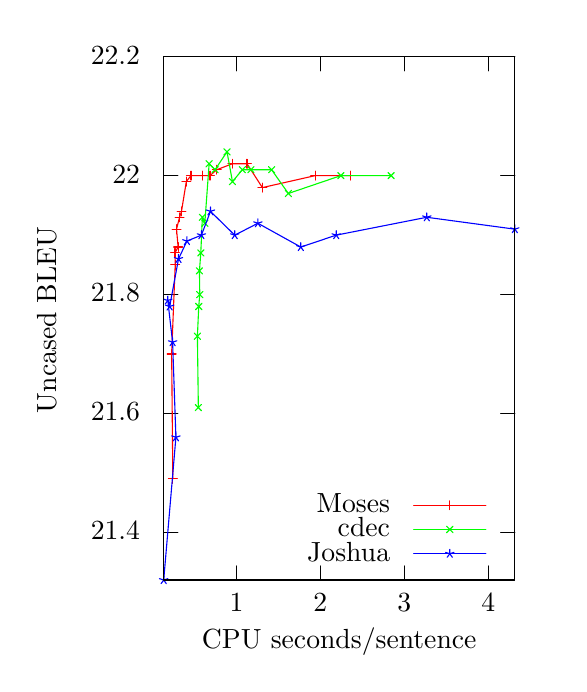
\begin{tikzpicture}[gnuplot]
%% generated with GNUPLOT 4.6p1 (Gentoo revision r0) (Lua 5.1; terminal rev. 99, script rev. 100)
%% Wed 03 Jul 2013 05:50:32 PM BST
\path (0.000,0.000) rectangle (6.700,8.000);
\gpcolor{color=gp lt color border}
\gpsetlinetype{gp lt border}
\gpsetlinewidth{1.00}
\draw[gp path] (1.688,1.589)--(1.868,1.589);
\draw[gp path] (6.147,1.589)--(5.967,1.589);
\node[gp node right] at (1.504,1.589) { 21.4};
\draw[gp path] (1.688,3.100)--(1.868,3.100);
\draw[gp path] (6.147,3.100)--(5.967,3.100);
\node[gp node right] at (1.504,3.100) { 21.6};
\draw[gp path] (1.688,4.610)--(1.868,4.610);
\draw[gp path] (6.147,4.610)--(5.967,4.610);
\node[gp node right] at (1.504,4.610) { 21.8};
\draw[gp path] (1.688,6.121)--(1.868,6.121);
\draw[gp path] (6.147,6.121)--(5.967,6.121);
\node[gp node right] at (1.504,6.121) { 22};
\draw[gp path] (1.688,7.631)--(1.868,7.631);
\draw[gp path] (6.147,7.631)--(5.967,7.631);
\node[gp node right] at (1.504,7.631) { 22.2};
\draw[gp path] (2.612,0.985)--(2.612,1.165);
\draw[gp path] (2.612,7.631)--(2.612,7.451);
\node[gp node center] at (2.612,0.677) { 1};
\draw[gp path] (3.678,0.985)--(3.678,1.165);
\draw[gp path] (3.678,7.631)--(3.678,7.451);
\node[gp node center] at (3.678,0.677) { 2};
\draw[gp path] (4.745,0.985)--(4.745,1.165);
\draw[gp path] (4.745,7.631)--(4.745,7.451);
\node[gp node center] at (4.745,0.677) { 3};
\draw[gp path] (5.811,0.985)--(5.811,1.165);
\draw[gp path] (5.811,7.631)--(5.811,7.451);
\node[gp node center] at (5.811,0.677) { 4};
\draw[gp path] (1.688,7.631)--(1.688,0.985)--(6.147,0.985)--(6.147,7.631)--cycle;
\node[gp node center,rotate=-270] at (0.246,4.308) {Uncased BLEU};
\node[gp node center] at (3.917,0.215) {CPU seconds/sentence};
\node[gp node right] at (4.679,1.935) {Moses};
\gpcolor{color=gp lt color 0}
\gpsetlinetype{gp lt plot 0}
\draw[gp path] (4.863,1.935)--(5.779,1.935);
\draw[gp path] (1.804,2.269)--(1.789,3.855)--(1.834,4.988)--(1.831,5.139)--(1.871,5.214)%
  --(1.851,5.441)--(1.889,5.592)--(1.914,5.667)--(1.975,6.045)--(2.034,6.121)--(2.178,6.121)%
  --(2.276,6.121)--(2.362,6.196)--(2.561,6.272)--(2.746,6.272)--(2.941,5.969)--(3.612,6.121)%
  --(4.065,6.121);
\gpsetpointsize{4.00}
\gppoint{gp mark 1}{(1.804,2.269)}
\gppoint{gp mark 1}{(1.789,3.855)}
\gppoint{gp mark 1}{(1.834,4.988)}
\gppoint{gp mark 1}{(1.831,5.139)}
\gppoint{gp mark 1}{(1.871,5.214)}
\gppoint{gp mark 1}{(1.851,5.441)}
\gppoint{gp mark 1}{(1.889,5.592)}
\gppoint{gp mark 1}{(1.914,5.667)}
\gppoint{gp mark 1}{(1.975,6.045)}
\gppoint{gp mark 1}{(2.034,6.121)}
\gppoint{gp mark 1}{(2.178,6.121)}
\gppoint{gp mark 1}{(2.276,6.121)}
\gppoint{gp mark 1}{(2.362,6.196)}
\gppoint{gp mark 1}{(2.561,6.272)}
\gppoint{gp mark 1}{(2.746,6.272)}
\gppoint{gp mark 1}{(2.941,5.969)}
\gppoint{gp mark 1}{(3.612,6.121)}
\gppoint{gp mark 1}{(4.065,6.121)}
\gppoint{gp mark 1}{(5.321,1.935)}
\gpcolor{color=gp lt color border}
\node[gp node right] at (4.679,1.627) {cdec};
\gpcolor{color=gp lt color 1}
\gpsetlinetype{gp lt plot 1}
\draw[gp path] (4.863,1.627)--(5.779,1.627);
\draw[gp path] (2.128,3.175)--(2.116,4.081)--(2.133,4.459)--(2.146,4.610)--(2.142,4.912)%
  --(2.159,5.139)--(2.179,5.592)--(2.210,5.516)--(2.265,6.272)--(2.340,6.196)--(2.492,6.423)%
  --(2.561,6.045)--(2.687,6.196)--(2.796,6.196)--(3.058,6.196)--(3.271,5.894)--(3.938,6.121)%
  --(4.576,6.121);
\gppoint{gp mark 2}{(2.128,3.175)}
\gppoint{gp mark 2}{(2.116,4.081)}
\gppoint{gp mark 2}{(2.133,4.459)}
\gppoint{gp mark 2}{(2.146,4.610)}
\gppoint{gp mark 2}{(2.142,4.912)}
\gppoint{gp mark 2}{(2.159,5.139)}
\gppoint{gp mark 2}{(2.179,5.592)}
\gppoint{gp mark 2}{(2.210,5.516)}
\gppoint{gp mark 2}{(2.265,6.272)}
\gppoint{gp mark 2}{(2.340,6.196)}
\gppoint{gp mark 2}{(2.492,6.423)}
\gppoint{gp mark 2}{(2.561,6.045)}
\gppoint{gp mark 2}{(2.687,6.196)}
\gppoint{gp mark 2}{(2.796,6.196)}
\gppoint{gp mark 2}{(3.058,6.196)}
\gppoint{gp mark 2}{(3.271,5.894)}
\gppoint{gp mark 2}{(3.938,6.121)}
\gppoint{gp mark 2}{(4.576,6.121)}
\gppoint{gp mark 2}{(5.321,1.627)}
\gpcolor{color=gp lt color border}
\node[gp node right] at (4.679,1.319) {Joshua};
\gpcolor{color=gp lt color 2}
\gpsetlinetype{gp lt plot 2}
\draw[gp path] (4.863,1.319)--(5.779,1.319);
\draw[gp path] (1.688,0.985)--(1.843,2.798)--(1.801,4.006)--(1.740,4.535)--(1.764,4.459)%
  --(1.876,5.063)--(1.983,5.290)--(2.167,5.365)--(2.282,5.667)--(2.590,5.365)--(2.884,5.516)%
  --(3.429,5.214)--(3.879,5.365)--(5.029,5.592)--(6.147,5.441);
\gppoint{gp mark 3}{(1.688,0.985)}
\gppoint{gp mark 3}{(1.843,2.798)}
\gppoint{gp mark 3}{(1.801,4.006)}
\gppoint{gp mark 3}{(1.740,4.535)}
\gppoint{gp mark 3}{(1.764,4.459)}
\gppoint{gp mark 3}{(1.876,5.063)}
\gppoint{gp mark 3}{(1.983,5.290)}
\gppoint{gp mark 3}{(2.167,5.365)}
\gppoint{gp mark 3}{(2.282,5.667)}
\gppoint{gp mark 3}{(2.590,5.365)}
\gppoint{gp mark 3}{(2.884,5.516)}
\gppoint{gp mark 3}{(3.429,5.214)}
\gppoint{gp mark 3}{(3.879,5.365)}
\gppoint{gp mark 3}{(5.029,5.592)}
\gppoint{gp mark 3}{(6.147,5.441)}
\gppoint{gp mark 3}{(5.321,1.319)}
\gpcolor{color=gp lt color border}
\gpsetlinetype{gp lt border}
\draw[gp path] (1.688,7.631)--(1.688,0.985)--(6.147,0.985)--(6.147,7.631)--cycle;
%% coordinates of the plot area
\gpdefrectangularnode{gp plot 1}{\pgfpoint{1.688cm}{0.985cm}}{\pgfpoint{6.147cm}{7.631cm}}
\end{tikzpicture}
%% gnuplot variables

\caption{\label{fig:model}Model scores and BLEU using cube pruning with pop limits ranging from 5 to 1000.}
\end{figure} 

This is likely due to the fact that in Moses and cdec, the calculation of language model state is delegated to the language model implementation~\cite{Heafield-left} which uses the internal data-structure of the language model to determine state (??? Ney paper from yrs ago). Joshua, on the other hand, uses the words in the left and right context to determine language model state. This results in more aggressive hypothesis recombination in Moses and cdec, leading to better model score.

%% (2013-07-08 Matt Post): This isn't true; Joshua does include the <s> and </s> symbols and allows
%% early combination with <s> (this was implemented last summer). Model scores between Moses and
%% Joshua are exact, now, with a properly converted model. The main decoder difference seems to be
%% that Joshua does not incorporate lefthand-side LM state collapsing for OOVs. I've commented out
%% the below because I think you'll want to include it but it will have to be moved somewhere
%% outside the discussion of differences from Joshua.

%% Secondly, the glue rule formulation in Moses and cdec is different from Joshua's. In Moses and cdec, the glue rule grammar is:
%% \begin{verbatim}
%%    S -> <s>
%%    S -> S X
%%    GOAL -> S </s> 
%% \end{verbatim}
%% where <s> and </s> are first-class words like any other. In Joshua, the glue rule grammar is:
%% \begin{verbatim}
%%    S -> X
%%    S -> S X
%%    GOAL -> <s> S </s> 
%% \end{verbatim}
%% In Moses and cdec formulation, glued hypotheses know that they are bound to the beginning of sentence <s>.  Therefore, their left language model state is empty and more hypotheses can recombine.  This is better than Joshua, where hypotheses are informed about <s> and </s> only after forming a complete sentence, so the left states are spuriously ambiguous.  Moreover, hypothesis score estimates are more accurate when they know about <s> earlier. Figure~\ref{fig:glue} shows the improvement in cdec by changing the glue rule formulation. This improvement was the direct result of research comparing the three decoders.

%% \begin{figure}[h]
%% \begin{center}
%% 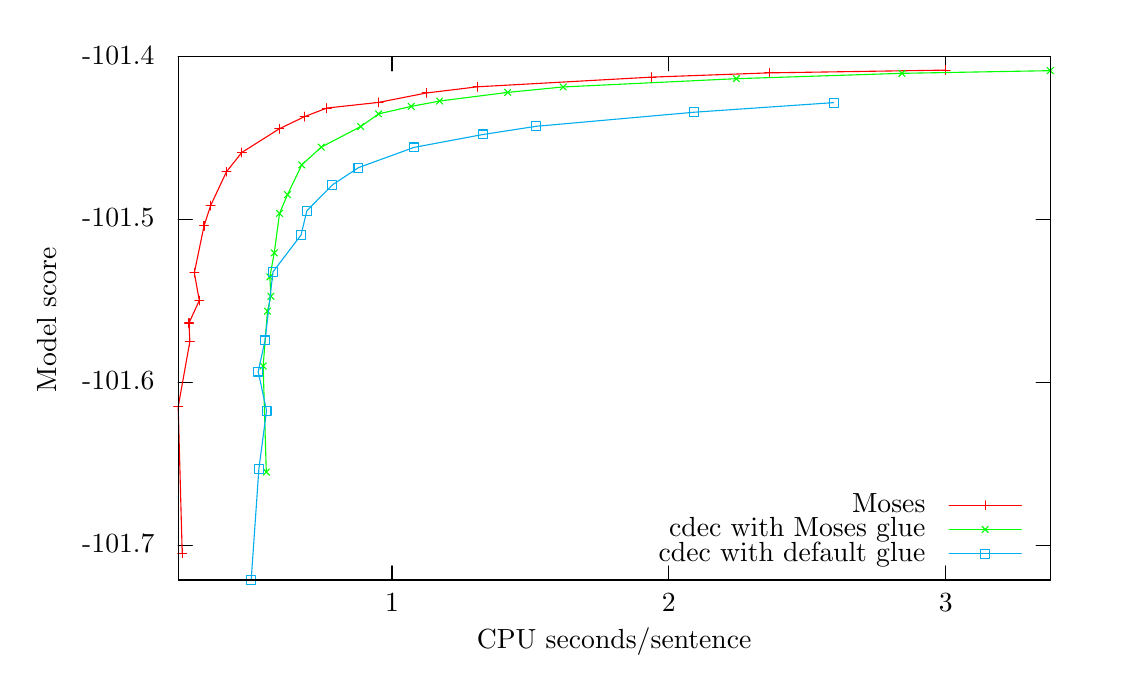
\begin{tikzpicture}[gnuplot]
%% generated with GNUPLOT 4.6p1 (Gentoo revision r0) (Lua 5.1; terminal rev. 99, script rev. 100)
%% Wed 03 Jul 2013 05:34:09 PM BST
\path (0.000,0.000) rectangle (13.500,8.000);
\gpcolor{color=gp lt color border}
\gpsetlinetype{gp lt border}
\gpsetlinewidth{1.00}
\draw[gp path] (1.872,1.429)--(2.052,1.429);
\draw[gp path] (12.947,1.429)--(12.767,1.429);
\node[gp node right] at (1.688,1.429) {-101.7};
\draw[gp path] (1.872,3.496)--(2.052,3.496);
\draw[gp path] (12.947,3.496)--(12.767,3.496);
\node[gp node right] at (1.688,3.496) {-101.6};
\draw[gp path] (1.872,5.564)--(2.052,5.564);
\draw[gp path] (12.947,5.564)--(12.767,5.564);
\node[gp node right] at (1.688,5.564) {-101.5};
\draw[gp path] (1.872,7.631)--(2.052,7.631);
\draw[gp path] (12.947,7.631)--(12.767,7.631);
\node[gp node right] at (1.688,7.631) {-101.4};
\draw[gp path] (4.587,0.985)--(4.587,1.165);
\draw[gp path] (4.587,7.631)--(4.587,7.451);
\node[gp node center] at (4.587,0.677) { 1};
\draw[gp path] (8.104,0.985)--(8.104,1.165);
\draw[gp path] (8.104,7.631)--(8.104,7.451);
\node[gp node center] at (8.104,0.677) { 2};
\draw[gp path] (11.620,0.985)--(11.620,1.165);
\draw[gp path] (11.620,7.631)--(11.620,7.451);
\node[gp node center] at (11.620,0.677) { 3};
\draw[gp path] (1.872,7.631)--(1.872,0.985)--(12.947,0.985)--(12.947,7.631)--cycle;
\node[gp node center,rotate=-270] at (0.246,4.308) {Model score};
\node[gp node center] at (7.409,0.215) {CPU seconds/sentence};
\node[gp node right] at (11.479,1.935) {Moses};
\gpcolor{color=gp lt color 0}
\gpsetlinetype{gp lt plot 0}
\draw[gp path] (11.663,1.935)--(12.579,1.935);
\draw[gp path] (1.923,1.326)--(1.872,3.185)--(2.020,4.014)--(2.009,4.249)--(2.140,4.535)%
  --(2.077,4.887)--(2.200,5.482)--(2.284,5.741)--(2.485,6.170)--(2.680,6.415)--(3.155,6.715)%
  --(3.476,6.870)--(3.760,6.979)--(4.418,7.051)--(5.028,7.171)--(5.673,7.249)--(7.886,7.372)%
  --(9.378,7.426)--(11.619,7.461);
\gpsetpointsize{4.00}
\gppoint{gp mark 1}{(1.923,1.326)}
\gppoint{gp mark 1}{(1.872,3.185)}
\gppoint{gp mark 1}{(2.020,4.014)}
\gppoint{gp mark 1}{(2.009,4.249)}
\gppoint{gp mark 1}{(2.140,4.535)}
\gppoint{gp mark 1}{(2.077,4.887)}
\gppoint{gp mark 1}{(2.200,5.482)}
\gppoint{gp mark 1}{(2.284,5.741)}
\gppoint{gp mark 1}{(2.485,6.170)}
\gppoint{gp mark 1}{(2.680,6.415)}
\gppoint{gp mark 1}{(3.155,6.715)}
\gppoint{gp mark 1}{(3.476,6.870)}
\gppoint{gp mark 1}{(3.760,6.979)}
\gppoint{gp mark 1}{(4.418,7.051)}
\gppoint{gp mark 1}{(5.028,7.171)}
\gppoint{gp mark 1}{(5.673,7.249)}
\gppoint{gp mark 1}{(7.886,7.372)}
\gppoint{gp mark 1}{(9.378,7.426)}
\gppoint{gp mark 1}{(11.619,7.461)}
\gppoint{gp mark 1}{(12.121,1.935)}
\gpcolor{color=gp lt color border}
\node[gp node right] at (11.479,1.627) {cdec with Moses glue};
\gpcolor{color=gp lt color 1}
\gpsetlinetype{gp lt plot 1}
\draw[gp path] (11.663,1.627)--(12.579,1.627);
\draw[gp path] (2.991,2.356)--(2.951,3.703)--(3.006,4.400)--(3.049,4.589)--(3.036,4.835)%
  --(3.092,5.139)--(3.159,5.641)--(3.260,5.879)--(3.441,6.257)--(3.689,6.483)--(4.190,6.744)%
  --(4.417,6.905)--(4.832,7.000)--(5.192,7.068)--(6.057,7.178)--(6.760,7.247)--(8.960,7.352)%
  --(11.063,7.420)--(12.947,7.454);
\gppoint{gp mark 2}{(2.991,2.356)}
\gppoint{gp mark 2}{(2.951,3.703)}
\gppoint{gp mark 2}{(3.006,4.400)}
\gppoint{gp mark 2}{(3.049,4.589)}
\gppoint{gp mark 2}{(3.036,4.835)}
\gppoint{gp mark 2}{(3.092,5.139)}
\gppoint{gp mark 2}{(3.159,5.641)}
\gppoint{gp mark 2}{(3.260,5.879)}
\gppoint{gp mark 2}{(3.441,6.257)}
\gppoint{gp mark 2}{(3.689,6.483)}
\gppoint{gp mark 2}{(4.190,6.744)}
\gppoint{gp mark 2}{(4.417,6.905)}
\gppoint{gp mark 2}{(4.832,7.000)}
\gppoint{gp mark 2}{(5.192,7.068)}
\gppoint{gp mark 2}{(6.057,7.178)}
\gppoint{gp mark 2}{(6.760,7.247)}
\gppoint{gp mark 2}{(8.960,7.352)}
\gppoint{gp mark 2}{(11.063,7.420)}
\gppoint{gp mark 2}{(12.947,7.454)}
\gppoint{gp mark 2}{(12.121,1.627)}
\gpcolor{color=gp lt color border}
\node[gp node right] at (11.479,1.319) {cdec with default glue};
\gpcolor{color=gp lt color 4}
\gpsetlinetype{gp lt plot 2}
\draw[gp path] (11.663,1.319)--(12.579,1.319);
\draw[gp path] (2.799,0.985)--(2.897,2.398)--(2.994,3.136)--(2.888,3.633)--(2.975,4.028)%
  --(3.076,4.899)--(3.433,5.368)--(3.506,5.675)--(3.830,6.003)--(4.161,6.222)--(4.865,6.479)%
  --(5.747,6.644)--(6.416,6.747)--(8.423,6.926)--(10.196,7.048);
\gppoint{gp mark 4}{(2.799,0.985)}
\gppoint{gp mark 4}{(2.897,2.398)}
\gppoint{gp mark 4}{(2.994,3.136)}
\gppoint{gp mark 4}{(2.888,3.633)}
\gppoint{gp mark 4}{(2.975,4.028)}
\gppoint{gp mark 4}{(3.076,4.899)}
\gppoint{gp mark 4}{(3.433,5.368)}
\gppoint{gp mark 4}{(3.506,5.675)}
\gppoint{gp mark 4}{(3.830,6.003)}
\gppoint{gp mark 4}{(4.161,6.222)}
\gppoint{gp mark 4}{(4.865,6.479)}
\gppoint{gp mark 4}{(5.747,6.644)}
\gppoint{gp mark 4}{(6.416,6.747)}
\gppoint{gp mark 4}{(8.423,6.926)}
\gppoint{gp mark 4}{(10.196,7.048)}
\gppoint{gp mark 4}{(12.121,1.319)}
\gpcolor{color=gp lt color border}
\gpsetlinetype{gp lt border}
\draw[gp path] (1.872,7.631)--(1.872,0.985)--(12.947,0.985)--(12.947,7.631)--cycle;
%% coordinates of the plot area
\gpdefrectangularnode{gp plot 1}{\pgfpoint{1.872cm}{0.985cm}}{\pgfpoint{12.947cm}{7.631cm}}
\end{tikzpicture}
%% gnuplot variables

%% \end{center}
%% \caption{Affect on model score by changing glue-rule formulation}
%% \label{fig:glue}
%% \end{figure}

\section{Conclusion}

???

\section*{Acknowledgements}

The research leading to these results has received funding from the European Union Seventh Framework Programme (FP7/2007-2013) under grant agreement 288487 (MosesCore).

% Bibliography
% ============
% You may either enter the bibliography manually, possibly making use of
% \label and \ref, or use BibTeX. The bibliography style is set
% automatically. You process the bibliography by BibTeX in the
% standard way and include it by:
\bibliography{mybib}

% If needed, add appendices here
%\section*{Appendix A: \ldots}

\correspondingaddress
\end{document}

% ======= Additional information ==========

% XeLaTeX
% =======
% The Prague Bulletin of Mathematical Linguistics is typeset by XeLaTeX.
% It is not required that you use XeLaTeX and the same fonts as will be used in the
% journal but it is better to do so if you could (so you have the same line and page breaks).
% If XeLaTeX is not available on your computer, you can even used standard LaTeX.

% Fonts
% =====
% In the printed version, fonts TeX Gyre Pagella (shipped with TeX Live 2008 or later)
% and DejaVu (http://dejavu.sourceforge.net/wiki/index.php/Main_Page)
% will be used. If you have XeLaTeX but not these fonts, you may need to install
% the fonts somewhere where your system (fontconfig) can find them. On Linux,
% try something like this:
% ln -s YOUR-TEXLIVE/2008/texmf-dist/fonts/opentype/public/ \
%  ${HOME}/.fonts/texlive-2008-otf-public
% If you are not able to install these fonts, you can instruct XeLaTeX
% to use its default fonts by \document[nofonts]{pbml}.

% If you want to typset examples in east Asian scripts, you have to use
% OpenType Unicode fonts that are freely redistributable and you have to
% include them with your article. If you must use nonfree or non-Unicode
% fonts, you must supply the examples as EPS or PDF with fonts embedded in
% the files (as the required subset).
% If encountering problems with the "bidi" package, contact pbml@ufal.mff.cuni.cz.

% Vector Graphics
% ===============
% The most portable graphics package is tikz which is a front end to pgf.
% This package is fully supported both in standard LaTeX and XeLaTeX.
% PSTricks is not currently available for XeLaTeX.

% Color Images
% ============
% The printed version of PBML does not allow color figures, so please convert
% all your figures to grayscale (or black&white), make sure they are legible
% and put them in a subdirectory called "grayscale".
% When specifying the filename in \includegraphics DO NOT include the
% subdirectory.
% Optionally, in addition to the default grayscale images, you can add also
% color versions of the figures to be published in the online version.
% Put such images in a subdirectory called "color" with the same filenames
% as the grayscale ones.
% To temporarily switch to color output and hypertext links, use
% \documentclass[color]{pbml}

% Including images and other files
% ===================================
% When loading the file you must use a relative path, never the full path.
% Load the images by \includegraphics
% and other files by \input, never use \include.
